% !TeX spellcheck = pl_PL 
\chapter{Analiza tematu}\label{ch:analiza}
\section{Podstawowe pojęcia}
\subsection{Definicja sieci przepływowej}\label{ssec:graphDef}
\emph{Sieć przepływowa} $ G=(V, E) $ jest grafem prostym skierowanym; strukturą, która składa się z dwóch zbiorów:
\begin{itemize}
	\item \textit{n}-elementowego zbioru wierzchołków $ V = \{v_1,v_2,...,v_n \}$
	\item \textit{m}-elementowwgo zbioru uporządkowanych łuków
	$$ E = \{e_1,e_2,...,e_m \},\quad \text{gdzie } e_i=(v_j,v_k);\quad i=1,...,m;\quad v_j,v_k\in V$$
	Każdy łuk jest parą wierzchołków należących do zbioru $ V $.
\end{itemize}
\emph{Grafem prostym} nazywamy taki graf w którym nie istnieją \emph{pętle}. Pętlą nazywamy łuk $ (v_j,v_k) $ dla którego $ v_j=v_k $. W sieci przepływowej wyróżnia się dwa wierzchołki: źródło $ s \in V $ oraz ujście $ t \in V $. W sieci przepływowej definiuje się ponadto \emph{funkcję przepustowości} $ c : E\rightarrow R_{\ge0}$ odwzorowującą zbiór łuków w zbiór liczb rzeczywistych. Dodatkowo, w celu uproszczenia dziedziny, zakłada się, że z każdego wierzchołka $ v\in V\backslash\{s, t\} $ istnieje ścieżka prowadząca ze źródła do ujścia. Założenie to ma zapewnić, że w rozpatrywanych sieciach będzie istniała co najmniej jedna ścieżka ze źródła do ujścia.
\emph{Stopniem wejściowym} wierzchołka nazywamy sumę łuków, jakie do niego wchodzą, a \emph{stopniem wyjściowym} sumę łuków, jakie z niego wychodzą.
\subsection{Definicja przepływu sieci}\label{ssec:flowDef}
\emph{Przepływem} w sieci przepływowej $ G $ jest funkcja $ f $, która odwzorowuje zbiór łuków w zbiór liczb rzeczywistych $ f : E \rightarrow R_{\ge0} $ i spełnia następujące założenia:
\begin{enumerate}
	\item Warunek przepustowości: $ \forall_{v_i, v_j\in V} : f(v_i, v_j) \le c(v_i, v_j) $.\\Przepływ w żadnym z łuków nie może przekroczyć jego przepustowości.
	\item Warunek skośnej symetryczności: $ \forall_{v_i, v_j\in V} : f(v_i, v_j) = -f(v_j, v_i) $.\\Przepływ w przeciwnym kierunku traktujemy tak jakby posiadał wartość ujemną.
	\item Warunek zachowania przepływu: $ \forall_{v\in V\backslash\{s, t\}} : \sum_{u\in V}f(v,u)=\sum_{u\in V}f(u,v) $.\\Suma przepływów wpływających do wierzchołka musi być równa sumie przepływów wypływających z niego.
\end{enumerate}
\subsection{Przepływ netto}\label{ssec:netto}
Przepływem netto nazywamy wartość funkcji przepływu $ f(v_i, v_j) $ pomiędzy wierzchołkami $ v_i $ oraz $ v_j $. Zgodnie z warunkiem skośnej symetryczności, wartość może być dodatnia lub ujemna. Dodatnia oznacza przepływ z wierzchołka $ v_i $ do wierzchołka $ v_j $, natomiast ujemna - w przeciwnym kierunku. Sieć przepływowa jest grafem skierowanym, więc dla dwóch wierzchołków może posiadać parę sąsiednich łuków. Poniższy przykład przedstawia istotę przepływu netto, jeżeli w obu sąsiadach istnieje niezerowy przepływ.
\begin{figure}[h]
	\centering
	\begin{subfigure}{0.25\textwidth}
		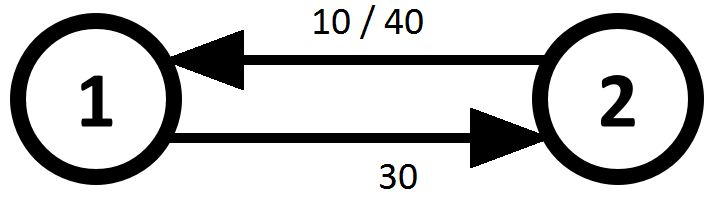
\includegraphics[width=0.9\linewidth]{./img/netto1.png} 
		\caption{}
		\label{fig:netto1}
	\end{subfigure}
	\begin{subfigure}{0.25\textwidth}
		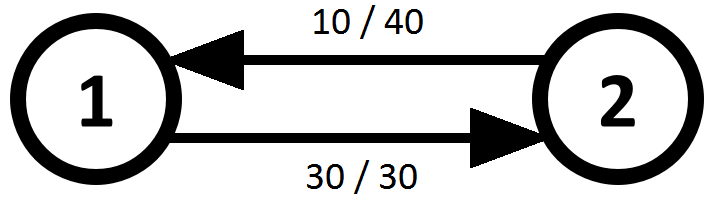
\includegraphics[width=0.9\linewidth]{./img/netto2.png}
		\caption{}
		\label{fig:netto2}
	\end{subfigure}
	\begin{subfigure}{0.25\textwidth}
		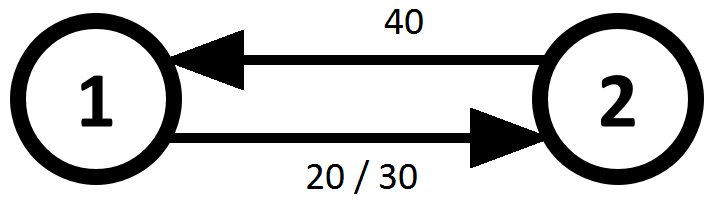
\includegraphics[width=0.9\linewidth]{./img/netto3.png}
		\caption{}
		\label{fig:netto3}
	\end{subfigure}
	\caption{Zobrazowanie przepływu netto}
	\label{fig:imageNetto}
\end{figure}\vfill
Na rysunku \ref{fig:netto1} istnieje przepływ z wierzchołka 2 do wierzchołka 1 o wartości 10, czyli $ f(2, 1) = 10 $. Zgodnie z warunkiem skośnej symetryczności $ f(1, 2) = f(2, 1) = -10 $. Można powiedzieć, że wierzchołek 2 opuszcza 10 jednostek materiału, które wpływają do wierzchołka 1. Na rysunku \ref{fig:netto2} pojawia się drugi przepływ, z wierzchołka 1 do wierzchołka 2 przepływa 30 jednostek. W tym przypadku wartość przepływu w istocie jest równa $ f(1,2)=-10 + 30=20 $. Jest to równoznaczne sytuacji, w której istnieje tylko przepływ 20 jednostek z wierzchołka 1 do wierzchołka 2, co przedstawia rysunek \ref{fig:netto3}. Przepływ z wierzchołka 2 do wierzchołka 1 zostaje zmniejszony do $ f(2, 1)=10-30=-20 $, co jest zgodne z warunkiem skośnej symetryczności.\cite{id:ZaawansowaneAlgorytmy}
\subsection{Maksymalny przepływ w sieci}
Wartość przepływu $ |f| $ w sieci jest definiowana jako suma przepływów netto wychodzących ze źródła $ \sum_{v\in V}{f(s, v)} $. Zgodnie z warunkiem zachowania przepływu, jest ona równa sumie wartości przepływów netto wpływających do ujścia $ \sum_{v\in V}{f(v, t)} $. Problem maksymalnego przepływu polega na znalezieniu maksymalnej wartości $ |f| $ w sieci przepływowej.\cite{id:ZaawansowaneAlgorytmy}
\subsection{Sieć residualna}\label{ssec:siecResidualna}
W celu wyznaczenia maksymalnego przepływu wprowadza się model \textit{sieci residualnej}. To dodatkowa sieć przepływowa utworzona na podstawie pierwotnej. Aby zwiększyć przepływ w sieci obserwuje się stan łuków - jeżeli przepustowość łuku nie jest zapełniona jego przepływem netto, to oznacza, że przepływ może być zwiększony. Wprowadza się w tym celu pojęcie \textit{przepustowości residualnej} $ c_f(v_i,v_j) $, definiowanej jako różnica przepustowości i przepływu netto.
$$ c_f(v_i,v_j)=c(v_i,v_j)-f(v_i,v_j) $$
Sieć residualną tworzy się w następujący sposób: dla każdego łuku $ (v_i,v_j) $ z sieci pierwotnej o przepływie $ f $ i przepustowości residualnej $ c_f $ tworzy się w sieci residualnej łuk $ (v_j,v_i) $ o przepustowości równej $ f $ oraz łuk $ (v_i,v_j) $ o przepustowości równej $ c_f $. Jeżeli istnieje łuk sąsiedni dokonuje się ujednolicenia przepływu netto zgodnie z \ref{ssec:netto}. W utworzonej tym sposobem sieci można zwiększyć przepływ jeżeli istnieje ścieżka ze źródła $ s $ do ujścia $ t $. Zobrazowanie utworzenia sieci residualnej znajduje na rysunku \ref{fig:residual}.
\begin{figure}[H]
	\centering
	\begin{subfigure}{0.45\textwidth}
		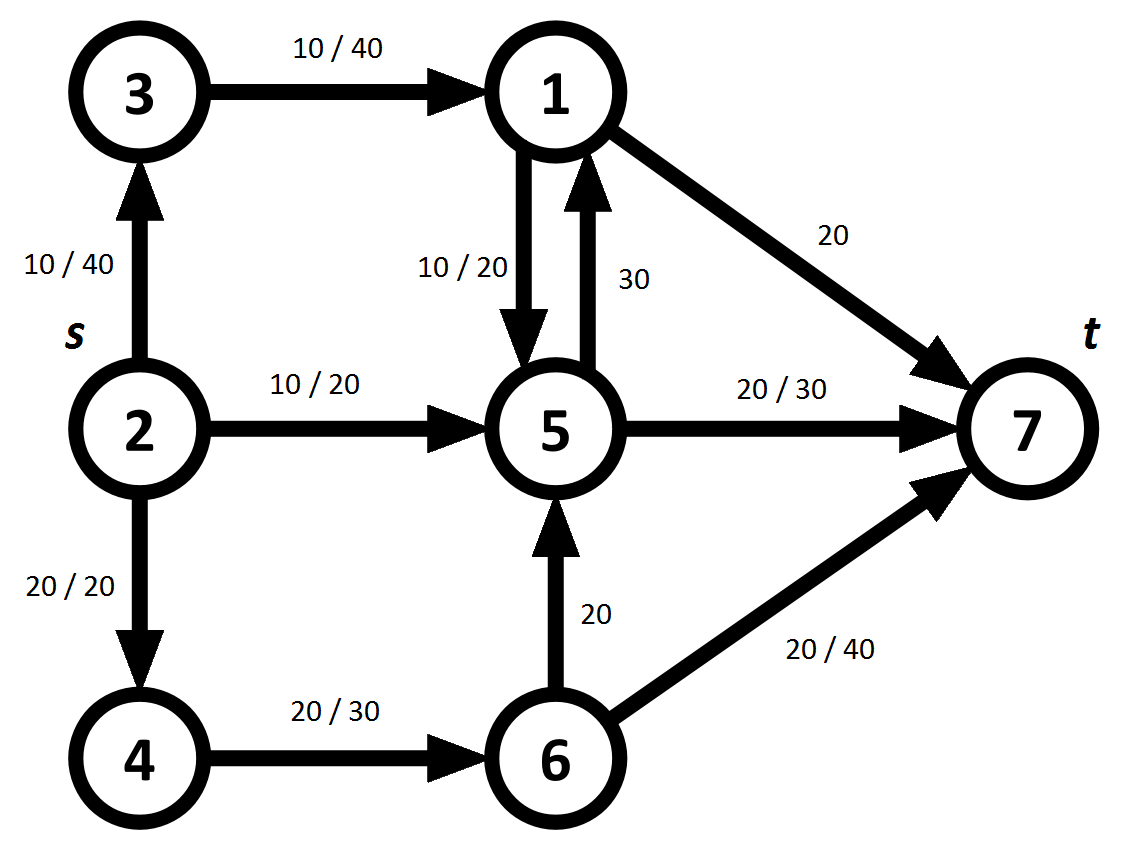
\includegraphics[width=0.9\linewidth]{./img/residual1.png} 
		\caption{}
		\label{fig:residual1}
	\end{subfigure}
	\begin{subfigure}{0.45\textwidth}
		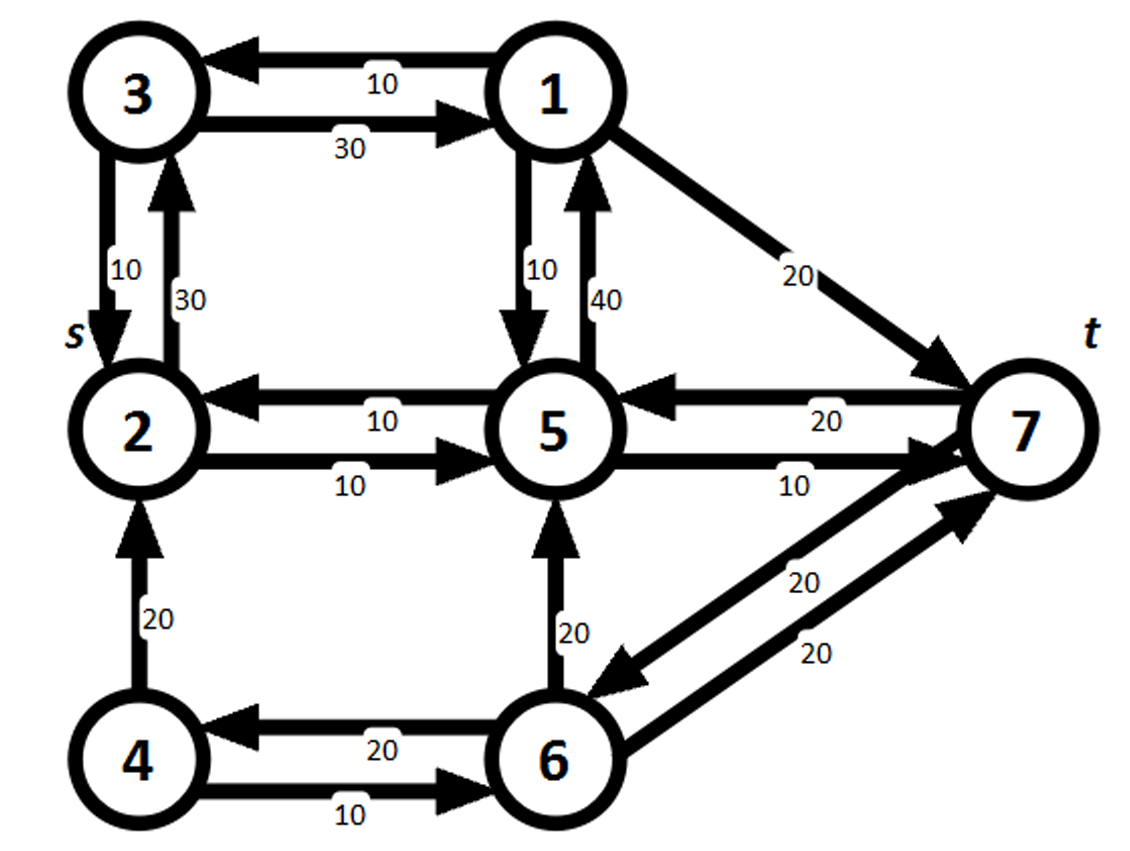
\includegraphics[width=0.9\linewidth]{./img/residual2.png}
		\caption{}
		\label{fig:residual2}
	\end{subfigure}
	\caption{Przykładowa sieć przepływowa i utworzona na jej podstawie sieć residualna}
	\label{fig:residual}
\end{figure}
Może się zdarzyć, że w sieci residualnej będą istnieć łuki, które nie istnieją w sieci pierwotnej lub będą posiadać przepustowość większą niż łuki odpowiadające w sieci pierwotnej. Należy wówczas w trakcie zwiększania przepływu wykorzystać \textit{przepływ zwrotny}, wynikający z warunku skośnej symetryczności, i zmniejszyć wartość przepływu netto w danym łuku.\newpage\indent
\textit{\textbf{Ścieżką powiększającą}} $ p $ w sieci residualnej nazywamy ścieżkę prostą (zbiór wierzchołków i łuków, gdzie każdy wierzchołek jest różny) ze źródła $ s $ do ujścia $ t $. Maksymalną wartością o jaką można zwiększyć przepływ dzięki niej jest najmniejsza przepustowość residualna spośród wszystkich łuków należących do tej ścieżki.
$$ c_f(p)=\min\{ c_f(v_i,v_j):\text{łuk } (v_i,v_j) \text{ należy do ścieżki }p\} $$
Jeżeli ścieżki powiększającej nie da się wyznaczyć w sieci residualnej, to oznacza, że aktualny przepływ $ f $ sieci pierwotnej jest maksymalny.
\subsection{Warstwowa sieć residualna}\label{ssec:WSR}
Inny rodzaj sieci residualnej, zapisujemy ją jako $ G_f^w=(V_f^w,E_f^w) $. Warstwowa sieć residualna oparta jest o ideę, że wyszukiwanie ścieżki powiększającej powinno odbywać się wyłącznie po najkrótszych możliwych ścieżkach, więc pewne wierzchołki i łuki nie będą do sieci należały. Niech $ d_{min}(v,u) $ będzie najkrótszą możliwą odległością między wierzchołkami $ v $ i $ u $ w sieci residualnej $ G=(V,E) $ ($ v,u\in V $), liczoną w liczbie łuków pośredniczących. Z sieci residualnej $ G $ zostają usunięte:
\begin{itemize}
	\item Wszystkie wierzchołki inne niż źródło, dla których minimalna odległość ze źródła jest większa niż odległość między źródłem, a ujściem.
	$$ V_f^w=V\backslash\{v\in V\backslash\{t\} : d_{min}(s,t)\le d_{min}(s,v)\} $$
	\item Łuki, dla których ścieżka ze źródła $ s $ do wierzchołka docelowego $ v_i $ jest mniejsza lub równa ścieżce ze źródła $ s $ do wierzchołka początkowego $ v_j $.
	$$ E_f^w=E\backslash\{(v_j,v_i)\in E : d_{min}(s,v_i)\le d_{min}(s,v_j)\} $$	
\end{itemize}
Powyższe warunki zapewniają, że każda ścieżka ze źródła $ s $ do dowolnego innego wierzchołka jest najkrótszą możliwą ścieżką. Pierwszy warunek gwarantuje nadmiarowych wierzchołków, a drugi łuków, które nie są częścią żadnej z najkrótszych ścieżek.
\begin{figure}[H]
	\centering
	\begin{subfigure}{0.40\textwidth}
		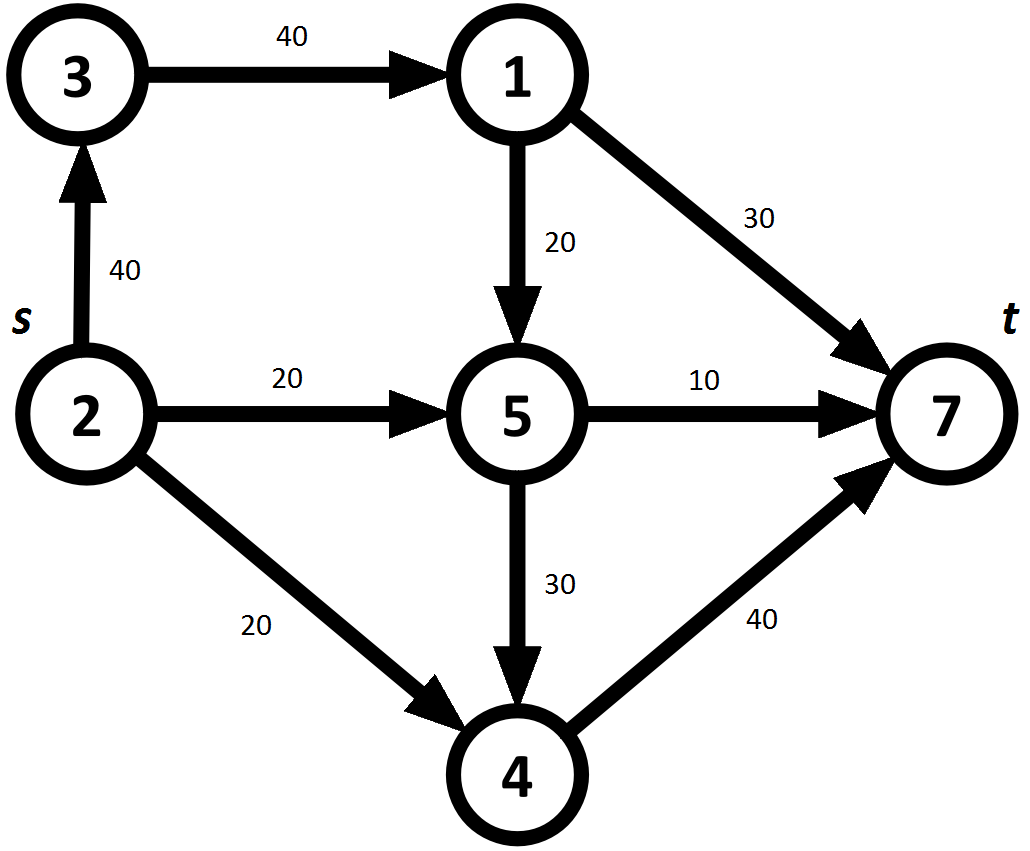
\includegraphics[width=0.9\linewidth]{./img/WSR1.png} 
		\caption{}
		\label{fig:wsr1}
	\end{subfigure}
	\begin{subfigure}{0.40\textwidth}
		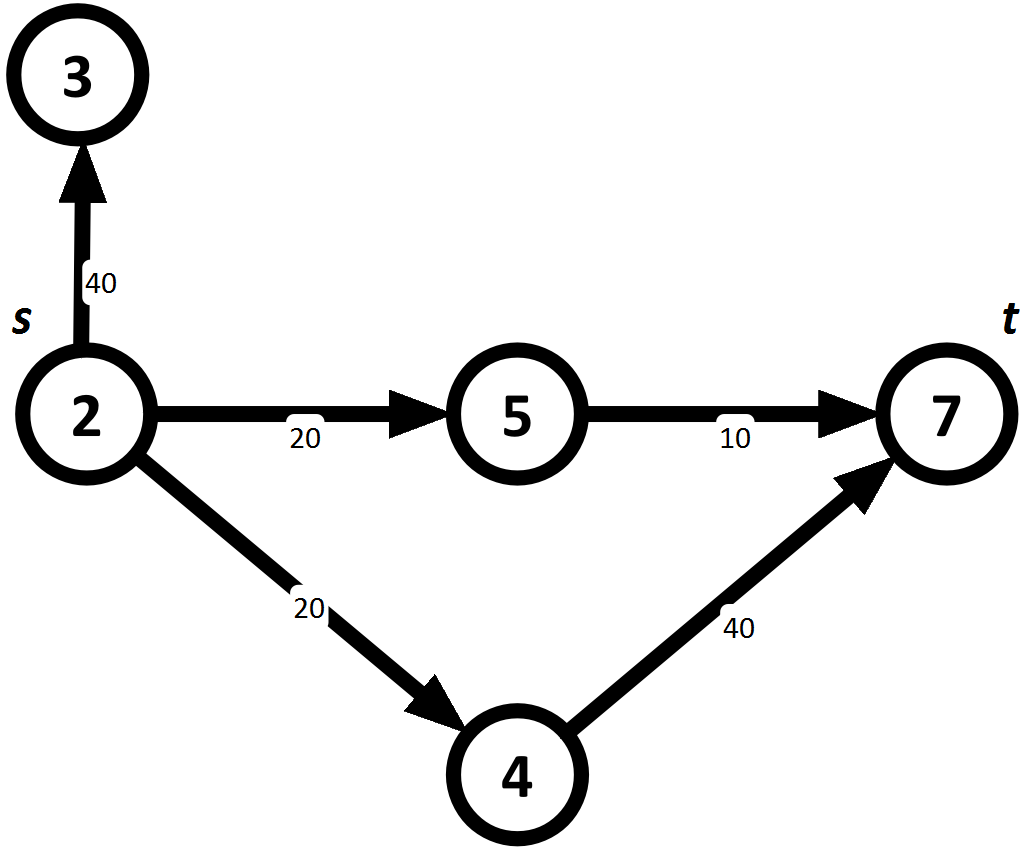
\includegraphics[width=0.9\linewidth]{./img/WSR2.png}
		\caption{}
		\label{fig:wsr2}
	\end{subfigure}
	\caption{Zobrazowanie różnicy między siecią residualną, a warstwową siecią residualną}
	\label{fig:wsr}
\end{figure}
Rysunek \ref{fig:wsr} prezentuje jak wygląda utworzenie warstwowej sieci residualnej (\ref{fig:wsr2}). W sieci residualnej (rys. \ref{fig:wsr1}) $ d_{min}(s,t)=2 $, ponieważ najkrótszą drogą jest $ s\rightarrow5\rightarrow t $. Zgodnie z pierwszym warunkiem został usunięty wierzchołek 1, ponieważ $ d_{min}(s, 1)=d_{min}(s,t)=2 $, a wraz z nim wszystkie łuki, które z niego wychodzą lub do niego prowadzą. Usunięty został również łuk $ (5,4) $, ponieważ $ d_{min}(s,4)=1 $ oraz $ d_{min}(s,5)=1 $, czyli droga ze źródła $ s $ do wierzchołka 4 nie będzie najkrótsza, gdy będzie przechodzić przez wierzchołek 5.\cite{id:ZaawansowaneAlgorytmy}
\section{Algorytmy znajdowania maksymalnego przepływu}\label{sec:analizaAlgorytmy}
\subsection{Algorytm Forda-Fulkersona}\label{ssec:FordFulkersonAnaliza}
\begin{algorithm}[H]
	\caption{Wyznaczenie maksymalnego przepływu algorytmem Forda-Fulkersona}\label{fordFulkersonPseudo}
	\begin{algorithmic}
		\Procedure{Znajdź maksymalny przepływ}{Sieć przepływowa $ G=(V, E) $}
			\State{Wykonaj sieć residualną $ G_f $ dla sieci przepływowej $ G $}
			\While{istnieje ścieżka powiększająca $ p $ w sieci $ G_f $}
				\State{Znajdź ścieżkę powiększającą $ p $ w sieci $ G_f $}
				\State{$ c_f(p) = min\{c_f(v_i,v_j):\text{łuk}\;(v_i,v_j)\text{ należy\:do\:ścieżki}\:p\} $}
				\ForAll{łuki $ (v_i,v_j)\in p$}
					\State{$ f[v_i,v_j] \text{ += } c_f(p) $}
					\State{$ f[v_j,v_i] = -f[v_i,v_j] $}
				\EndFor
				\State{Wykonaj sieć residualną $ G_f $ dla sieci przepływowej $ G $}
			\EndWhile\State{\Return{f}}
		\EndProcedure
	\end{algorithmic}
\end{algorithm}\noindent
Idea wyznaczania maksymalnego przepływu oparta jest o iteracyjne tworzenie sieci residualnej i szukania w niej ścieżki powiększającej. W każdej iteracji:
\begin{itemize}
	\item tworzona jest sieć residualna $ G_f $ na podstawie sieci przepływowej $ G $ i jej aktualnego przepływu,
	\item znajdowana jest ścieżka powiększająca $ p $ w sieci residualnej,
	\item wartością powiększającą $ c_f(p) $ jest najmniejsza przepustowość residualna wśród łuków w ścieżce $ p $,
	\item dla każdego łuku $ (v_i,v_j) $ ze ścieżki powiększającej $ p $ zwiększ przepływ w odpowiadającym łuku w sieci przepływowej $ G $ o wartość $ c_f(p) $,
	\item dla każdego łuku sąsiadującego z łukiem $ (v_i,v_j) $ utwórz przepływ zwrotny. 
\end{itemize}
W definicji algorytmu nie jest podany sposób wyznaczania ścieżki powiększającej, ponieważ nie ma on wpływu na wynik - przepływ zawsze jest maksymalny, z kolei wybór ma wpływ na czas wykonywania algorytmu \cite{id:ZaawansowaneAlgorytmy}, \cite{id:IntroductionToAlgorithms}. Przykładowe działanie algorytmu znajduje się w dodatku \ref{add:C}.
\subsection{Wykorzystanie przepływu blokującego}\label{ssec:blockingFlowAnaliza}
\textbf{\textit{Przepływem blokującym}} $ f_b $ nazywamy taki przepływ w sieci, dla którego każda ścieżka ze źródła do ujścia posiada co najmniej jeden łuk nasycony. \textbf{\textit{Łukiem nasyconym}} nazywamy taki łuk $ (v_i,v_j) $, którego przepływu netto nie można już zwiększyć, $ c(v_i,v_j)=f(v_i,v_j) $. Wykorzystanie \textit{warstwowej sieci residualnej} \ref{ssec:WSR} zapewnia, że każda ścieżka powiększająca w tej sieci będzie posiadać co najmniej jeden łuk nasycony. Dzięki temu można łatwo wyznaczyć przepływ blokujący w tej sieci szukając wszystkich możliwych ścieżek powiększających i składając je w jeden przepływ $ f_b $. Zwiększenie przepływów netto w sieci pierwotnej traktujemy dokładnie tak samo jak dla zwykłej ścieżki powiększającej \ref{ssec:netto} \cite{id:ZaawansowaneAlgorytmy}.\\\indent
Działanie algorytmu poszukującego maksymalnego przepływu w sieci jest analogiczne do  \ref{ssec:FordFulkersonAnaliza}, ale zamiast sieci residualnej tworzy się warstwową sieć residualną, a zamiast ścieżki powiększającej - przepływ blokujący.
\begin{algorithm}[H]
	\caption{Wyznaczenie maksymalnego przepływu z wykorzystaniem przepływu blokującego} \label{blockingFlowPseudo}
	\begin{algorithmic}
		\Procedure{Znajdź maksymalny przepływ}{Sieć przepływowa $ G=(V, E) $}
		\State{Wykonaj warstwową sieć residualną $ G_f^w $ dla sieci przepływowej $ G $}
		\While{istnieje ścieżka ze źródła do ujścia w sieci $ G_f^w $}
			\State{Znajdź przepływ blokujący $ f_b $ w sieci $ G_f^w $}
			\State{Zwiększ przepływ $ f $ w sieci $ G $ o wartość $ f_b $}
			\State{Wykonaj warstwową sieć residualną $ G_f^w $ dla sieci przepływowej $ G $}
		\EndWhile\space\Return{f}
		\EndProcedure
	\end{algorithmic}
\end{algorithm}
\subsection{Algorytm Dinica}\label{ssec:dinicAnaliza}
Ten algorytm wykorzystuje wyznaczanie maksymalnego przepływu za pomocą warstwowej sieci residualnej oraz przepływu blokującego, opisane w \ref{ssec:blockingFlowAnaliza}. Definiuje sposób wyznaczania przepływu blokującego.
\begin{algorithm}[H]
	\caption{Wyznaczenie przepływu blokującego algorytmem Dinica}\label{dinicPseudo}
	\begin{algorithmic}
		\Procedure{Wyznacz przepływ blokujący}{Warstwowa sieć residualna $ G_f^w=(V_f^w,E_f^w) $}
			\While{istnieje ścieżka powiększająca $ p $ w sieci $ G_f^w $}
				\State{Wyznacz ścieżkę powiększającą $ p $ w sieci $ G_f^w $}
				\State{$ c_f(p) = min\{c_f(v_i,v_j):\text{łuk}\;(v_i,v_j)\text{ należy\:do\:ścieżki}\:p\} $}
				\ForAll{łuki $ (v_i,v_j) $ należące do ścieżki $ p $}
					\State{$ f_b[v_i,v_j] \text{ += } c_f(p)$}
					\State{$ c_f[v_i,v_j] \text{ }-\text{= } c_f(p)$}
					\If{$ c_f[v_i,v_j]=0 $}
						\State{Usuń łuk $ (v_i,v_j) $ z sieci $ G_f^w $}
					\EndIf
				\EndFor
				\State{Usuń wierzchołki $ v\in V_f^w $, których stopień wejściowy lub stopień wyjściowy jest równy 0}
			\EndWhile\State{\Return{$ f_b $}}
		\EndProcedure
	\end{algorithmic}
\end{algorithm}\noindent
Idea polega na usuwaniu w każdej iteracji łuków nasyconych z warstwowej sieci residualnej, a następnie wszystkich wierzchołków, które mają zerowy stopień wejściowy lub wyjściowy. Konstrukcja sieci zapewnia, że przy wyznaczaniu kolejnej ścieżki powiększającej w przepływie blokującym na pewno nie będzie ona przechodzić przez łuki nasycone oraz wierzchołki, które nigdzie nie prowadzą lub nie można do nich dojść, więc można je usunąć w celu przyspieszenia obliczeń \cite{id:ZaawansowaneAlgorytmy}. Przykładowe działanie algorytmu znajduje się w dodatku \ref{add:dinicExample}.
\subsection{Algorytm MKM}\label{ssec:mkmAnaliza}
Podobnie jak algorytm Dinica, ten algorytm wykorzystuje przepływ blokujący do wyznaczania maksymalnego przepływu (rozdział  \ref{ssec:blockingFlowAnaliza}) i jedyną różnicą jest definicja metody tworzenia go. Algorytm MKM do utworzenia przepływu blokującego nie używa ścieżek powiększających, ale wykorzystuje pojęcie \textit{\textbf{potencjału przepływowego wierzchołka}} $ p_f(v) $.
$$ p_f(v)=\min\{p_f^{we}(v),p_f^{wy}(v)\},\quad p_f^{we}(v)=\sum_{u\in V}{c(u,v)},\quad p_f^{wy}(v)=\sum_{u\in V}{c(v,u)} $$
Przez $ p_f^{we}(v) $ określony jest potencjał wejściowy wierzchołka $ v $ (suma przepustowości łuków wchodzących), a przez $ p_f^{wy}(v) $ potencjał wyjściowy wierzchołka $ v $ (suma przepustowości łuków wychodzących). Potencjał przepływowy jest mniejszą z tych dwóch wartości, czyli określa maksymalną wartość przepływu, jaka może zostać przetransportowana przez wierzchołek. Definiuje się ponadto, że $ p_f^{we}(s)=\infty $ oraz $ p_f^{wy}(t)=\infty $  \cite{id:ZaawansowaneAlgorytmy}.
\begin{algorithm}[H]
	\caption{Wyznaczenie przepływu blokującego algorytmem MKM}\label{mkmPseudo}
	\begin{algorithmic}
		\Procedure{Wyznacz przepływ blokujący}{Warstwowa sieć residualna $ G_f^w=(V_f^w,E_f^w) $}
			\State{Oblicz dla każdego wierzchołka $ v \in V_f^w$ potencjały $ p_f^{we}(v),\;p_f^{wy}(v),\;p_f(v) $}
			\Repeat
				\State{Znajdź wierzchołek $ v\in V_f^w $ o najmniejszym potencjale przepływowym $ p_f(v) $}
				\State{Utwórz ścieżkę $ v\rightarrow t $, prześlij nią $ p_f(v) $ jednostek i uaktualnij $ f_b $}
				\State{Utwórz ścieżkę $ s\rightarrow v $, prześlij nią $ p_f(v) $ jednostek i uaktualnij $ f_b $}
				\State{Oblicz dla każdego wierzchołka $ v \in V_f^w$ potencjały $ p_f^{we}(v),\;p_f^{wy}(v),\;p_f(v) $}
				\State{Usuń z sieci $ G_f^w$ wszystkie wierzchołki $ v \in V_f^w$ dla których $ p_f(v)=0 $}
			\Until{$ s\not\in V_f^w $ lub $ t\not\in V_f^w $}
			\State{\Return{$ f_b $}}
		\EndProcedure
	\end{algorithmic}
\end{algorithm}\vfill
W każdej iteracji w warstwowej sieci residualnej $ G_f^w $ poszukuje się wierzchołka $ v $ o najmniejszym potencjale przepływowym. Następnie tworzy się dwie ścieżki: prowadzącą ze źródła $ s $ do wierzchołka $ v $ oraz z wierzchołka $ v $ do ujścia $ t $, które razem tworzą ścieżkę powiększającą przechodzącą przez wierzchołek $ v $. Następuje zwiększenie przepływu w $ G_f^w $, a następnie usunięcie wszystkich wierzchołków o zerowym potencjale przepływowym i w konsekwencji łuków wchodzących i wychodzących z tych wierzchołków. Algorytm kończy pracę gdy zostanie usunięte źródło $ s $ lub ujście $ t $. Przykładowe działanie algorytmu znajduje się w dodatku \ref{add:mkmExample}.

\section{Wykorzystane technologie}
\subsection{Język programowania}\label{ssec:technologieJezyk}
Aplikacja ma mieć charakter edukacyjny, więc na pierwszym planie nie stała efektywność wykonywania samych algorytmów, ale sposób prezentacji ich działania. Użytkownik korzystający z aplikacji powinien móc odwzorować w niej książkowy przykład sieci przepływowej oraz móc zaobserwować jak każdy z interesujących go algorytmów wykonuje swoją pracę krok po kroku, jakie wprowadza zmiany w jego sieci i dlaczego. W tym celu zdecydowano się na platformę graficzną \textbf{\textit{Qt}} oraz język programowania \textbf{\textit{C++}}. Qt oferuje możliwość tworzenia prostych kształtów geometrycznych w grafice wektorowej; sieć tworzona przez użytkownika będzie tak samo czytelna w dowolnym przybliżeniu. Platforma Qt umożliwia również proste i wygodne w użyciu tworzenie okręgów, linii, łączenie ich w większe konstrukcje, zmiany parametrów, obsługę zdarzeń itp. Dzięki niej da się utworzyć pole edycyjne rysunku podobne do tych z takich aplikacji desktopowych jak \textit{Inkscape} lub \textit{Photoshop} oraz wygodne dla użytkownika tworzenie sieci przepływowych przy pomocy kilku prostych narzędzi. Wybrana przez mnie wersja Qt to \emph{Open Source}.
\subsection{Środowisko deweloperskie}
Decydując się na język C++ i platformę Qt istniała możliwość pracy w dwóch środowiskach IDE: \textit{Visual Studio 2013} z wtyczką do Qt oraz \textit{Qt Creator}. Zdecydowano się na środowisko \textit{\textbf{Visual Studio 2013}}, aby móc w trakcie pracy skorzystać ze wszystkich dobrodziejstw kontroli kodu i debugowania, jakie oferuje produkt firmy Microsoft. Nie można było korzystać z najnowszego Visual Studio 2015, ponieważ w tym czasie wtyczka zespalająca VS z Qt, \textbf{\textit{Qt Visual Studio Add-in 1.2.4}}, nie obsługiwała jeszcze tej wersji. Konsekwentnie aplikacja została napisana w \textit{\textbf{Qt 5.5}} oraz skompilowana pod kompilatorem \textbf{\textit{MSVC v12.0 x64}} na systemy Windows. Przez pewien czas nad rozwojem aplikacji pracowano z wtyczką \textbf{\textit{Resharper C++}} (wersja próbna), która znacznie usprawniała pracę w środowisku Visual Studio. Tworząc okna i okienko dialogowe, z których korzysta aplikacja, korzystano dodatkowo z \textbf{\textit{Qt Designer}}a, który dawał możliwość komfortowego projektowania GUI w na tę platformę. Do pomocy ze statyczną analizą kodu korzystano dodatkowo z aplikacji \textbf{\textit{Cppcheck}}.
\subsection{Format plików przy serializacji}
Jednym z podstawowych wymagań aplikacji jest możliwość zapisu i odczytu sieci przepływowych z plików zewnętrznych. Zdecydowano się na zapisywanie ich do formatu \textbf{\textit{XML}} bez szyfrowania pliku za pomocą funkcji mieszających. Format jest bardzo powszechny i posiada wsparcie w większości języków programowania, czy to w postaci bibliotek czy dzięki różnym platformom. Format pliku jest czytelny zarówno dla maszyny, jak i dla człowieka. Zmiany można wprowadzać edytując sam plik, dzięki temu możliwe jest wprowadzanie drobnych zamian zarówno przez użytkownika, który chciałby wprowadzić pewne zmiany bez otwierania aplikacji, jak i dla dewelopera, który chciałby testować i debugować w ten sposób działanie kodu parsującego.
\subsection{Kontrola wersji}\label{ssec:kontrolaWersji}
Pracując nad aplikacją była potrzeba, aby mieć repozytorium kodu, na którym trzymano by kod źródłowy pracy inżynierskiej oraz można by obserwować i kontrolować jej rozwój, jak również móc wrócić do poprzednich wersji w przypadku popełnienia błędów. Zdecydowano się na repozytorium w systemie \textbf{\textit{Git}} z wykorzystaniem klienta \textbf{\textit{Bitbucket}}.